In the previous chapter, we have introduced Conditional ICA, an efficient generative
model for task and rest fMRI data.
In this chapter, we first show that the generative model of resting state data shipped in Conditional ICA produces samples that neither linear nor non-linear classifiers are able to distinguish.
% 
Then we benchmark Conditional ICA as a generative model of task data against
various augmentation methods  on their
ability to improve classification accuracy on a large task fMRI dataset.
We find that Conditional ICA yields highest accuracy improvements.
In particular Conditional ICA outperforms GANs and conditional GANs~\cite{mirza2014conditional} while being much easier to optimize and interpret. 
Lastly, we show on 8 different datasets that the use of Conditional ICA results in systematic improvements in classification accuracy ranging from 1\% to 5\%.

\section{Dataset, data augmentation baselines and classifiers used}
\label{sec:condica:datasets}
The unmixing matrices are learned on the rest HCP
dataset~\cite{van2013wu} using 200 subjects.
These data were used after standard
preprocessing, including linear detrending, band-pass filtering
($[0.01, 0.1]Hz$) and standardization of the time courses.
The other 8 datasets~\cite{van2013wu, shafto2014cambridge,
  orfanos2017brainomics, pinel2019functional, pinel2007fast, pinel2013genetic,
  poldrack2016phenome, pinel2013genetic} are obtained from the Neurovault repository~\cite{gorgolewski2015neurovault}.
The classes used in each of these datasets correspond to the activation maps
related to contrasts (such as ``face vs tools'')
present in the set of tasks of each dataset. In table~\ref{fig:dataset:tab}, we
give references to the datasets used as well as the total number of samples
(subjects), the size of train and test sets in each of the cross validation
splits and the number of classes in each dataset. 

\begin{table}
\begin{center}
\begin{tabular}{c|c|c|c}
\hline
Dataset & Subjects, & Train/Test & Neurovault \\
 & classes  &  & collection 
\\ \hline
hcp~\cite{van2013wu}  & 787, 23 & 100/687  &  4337
\\
cam-can \cite{shafto2014cambridge}  & 605, 5 & 100/505  &  4342
\\
brainomics \cite{orfanos2017brainomics}  & 94, 19 & 50/44  &   4341
\\
archi \cite{pinel2019functional}  & 78, 30 & 40/38  &  4339
\\
la5c \cite{poldrack2016phenome}  & 191, 24 & 100/91  &  4343
\\
pinel2012archi \cite{pinel2019functional} & 76, 10 & 40/36  &  1952
\\
pinel2009twins \cite{pinel2013genetic}  & 65, 12 & 35/30  &  1952
\\
pinel2007fast \cite{pinel2007fast} & 133, 10 & 70/63  &  1952
\\\hline\hline
\end{tabular}
\end{center}
\caption{\textbf{Datasets used in the experiments.} The table provides
  references to the datasets that were used for our experiments, with
  the number of subjects, the number of classes, the number of subjects in train
  and test set in each cross validation split and the collection number in Neurovault}
  \label{fig:dataset:tab}
\end{table}


We consider 5 alternative
augmentation methods: \emph{ICA}, \emph{Covariance}, \emph{ICA + Covariance}, \emph{GANs} and \emph{CGANs}.
%
When no augmentation method is applied we use the label \emph{Original}.

The \emph{ICA} method applies ICA to $X^{task}$ to generate unmixing matrices $W^{task}$ and
components $S^{task}=  W^{task} X^{task}$.
%
To generate a sample $\tilde{\xb}_c$ from class $c$, we sample
independently from each component restricted to the samples of class $c$ yielding $\tilde{\sbb}^{task}_c$ and mix the data: $\tilde{\xb}_c = (W^{task})^{\dagger}
\tilde{\sbb}^{task}_c$.
%

The \emph{Covariance} method generates a new sample of
synthetic data in class $c$ by sampling from a Multivariate Gaussian
with mean $\mub_c$ and covariance $\Sigma$, where $\mub_c$ is the
class mean and $\Sigma$ is the covariance of centered task data
estimated using Ledoit-Wolf method.
%
In brief, it assumes normality of the data per class.

The \emph{ICA + Covariance} method combines the augmentation
methods \emph{ICA} and \emph{Covariance}: samples are drawn following
the ICA approach, but with some additive non-isotropic Gaussian noise.
%
As in \emph{ICA} we estimate $W^{task}$ and $S^{task}$ from
$X^{task}$ via ICA.
%
Then we consider $R_{task} = X_{task} - W_{task} S_{task}$ and estimate the
covariance $\Sigma_R$ of $R_{task}$ via LedoitWolf's method.
%
We then generate a data sample $\tilde{\xb}_c$ from class $c$ as with ICA and add
Gaussian noise $\tilde{\nb} \sim \mathcal{N}(0,\Sigma_R)$.
%
Samples are thus generated as $\tilde{\xb}_c + \tilde{\nb}$.

\emph{GANs} are used in the unsupervised setting (resting state fMRI generation)
while \emph{CGANs} can generate fake data from a given class (task fMRI
generation). In the GANs or CGANs method, the generator and discriminator have a mirrored architecture with 2 fully connected hidden layer of size (256 and 512).  The number of epochs, batch size, momentum and learning rate are set to 20k, 16, 0.9, 0.01 and we use the Leaky RELU activation function.

We evaluate the performance of augmentation methods through the use of classifiers: logistic regression (LogReg), linear
discriminant analysis with Ledoit-Wold estimate of covariance (LDA) perceptron
with two hidden layers (MLP) and random forrests (RF).
The hyper-parameters in each classifier are optimized through an internal 5-Fold
cross validation. We set the number of iterations in each classifier so that
convergence is reached. The exact specifications are given in table~\ref{fig:classifiers:tab}.

\begin{table}
  \begin{tabular}{ p{.11\textwidth} | p{.3\textwidth} |p{.5\textwidth}}
\hline
  Methods & Optimizer & Hyper-parameters \\
  \hline
LogReg & L-BFGS \newline ($20~000$ iterations) & inverse $L_2$ regularization
strength \newline in $\{0.0001, 0.001, 0.01, 0.1, 1 \}$ \\
  \hline
LDA  & Least-squares solver & Estimation of covariance \newline using Ledoit-Wolf's
                              method \\
  \hline
  RF &  - &  Default parameters in sklearn \\
  \hline
MLP  & Adam \newline ($20~000$ iterations, \newline momentum: $0.9$, \newline
batch size: $32$, \newline learning
       rate: $0.0001$) & $ReLU$ activation function, fully connected
                         architecture with two hidden layers both of size $1024$, L2
                         penalty coefficient: $10^{-5}$
\caption{\textbf{Optimizers and hyper-parameters of classifiers} For each classifier, we give the optimization method used as well as the value of hyper-parameters.}\label{fig:classifiers:tab} 
\end{tabular}
\end{table}


 
\section{Distinguish fake from real HCP resting state data}
This experiment is meant to assess the effectiveness of the data
augmentation scheme in producing good samples.
Data augmentation methods are trained on 200 subjects taken from HCP rest fMRI
dataset which amounts to $960k$ samples (4800
per individual). Then synthetic
data corresponding to $200$ synthetic subjects are produced, yielding
$960k$ fake samples and various classifiers are trained to distinguish fake from
real data using 5-Fold cross validation. The cross-validated accuracy is shown
in table~\ref{tab2}.
Interestingly, we observe a dissociation between linear models (LogReg
and LDA) that fail to discriminate between generated and actual data,
and non-linear models (MLP and RF) that can discriminate samples from
the alternative augmentation methods.
%
By contrast, all classifiers are at chance when Conditional ICA is used.

\begin{table}
\begin{center}
\begin{tabular}{c|cccc}
\hline
Models & LDA  & LogReg & Random Forest &  MLP 
\\ \hline
ICA   & 0.493 & 0.500 & 0.672 &  0.697
\\
Covariance   & 0.473 & 0.461 & 0.610 &  0.626
\\
ICA + Covariance   & 0.509 & 0.495 & 0.685 &  0.706
\\
GANs   & 0.501 & 0.498 & 0.592 &  0.607
% \\
% CGANs   & 0.498 &  0.493 & 0.579 & 0.604
\\\hline
\textbf{Conditional ICA}  & 0.503 & 0.489 & 0.512 &  0.523
\\\hline\hline
\end{tabular}
\end{center}
  \caption{\textbf{Distinguish fake from real HCP resting state data}
    We use HCP resting state data from $n=200$ subjects ($960k$ samples) and produce an equally
    large amount of fake data ($960k$ samples) using data augmentation methods.
    The table shows the 5-fold cross validated accuracy obtained with various
    classifiers. When Conditional ICA is used, all classifiers are at chance.
    %
    }\label{tab2}
\end{table}
%
\section{Comparing augmentation methods based on classification accuracy on task
  HCP dataset}
In order to compare the different augmentation methods, we measure their 
relative benefit in the context of multi-class classification.
We use 787 subjects from the HCP task dataset that contains 23 classes and
randomly split the dataset into a train set that contains 100 subjects and a test set
that contains 687 subjects. In each split we train augmentation methods on the
train set to generate fake samples corresponding to $200$ subjects.  
These samples are then appended to the train set, resulting in an
augmented train set on which the classifiers are trained. Results, displayed in
table~\ref{condica:tab3}, show that Conditional ICA always yields a higher accuracy
than when no augmentation method is applied. The gains are over 1\% on all
classifiers tested excepts with the random forest classifier which yields much
lower accuracy than other methods.
%
By contrast, ICA+Covariance and ICA lead to a decrease in accuracy
while the Covariance approach leads to non-significant
gains.
%

\begin{table}
  \setlength{\tabcolsep}{0.23em}
  % {\renewcommand{\arraystretch}{1}% for the vertical padding
  \begin{center}
    \begin{tabular}{c|c|c|c | c}
      \hline
      Models & LDA & LogReg & MLP& RF\\
      \hline
      Original           & 0.893 & 0.874 &  0.779 &0.782 \\
    ICA                & 0.814 & 0.840 &  0.803 &0.778\\
    Covariance         & 0.895 & 0.876 &  0.819 &0.780\\
    ICA + Covariance   & 0.816 & 0.840 &  0.815 &0.780\\
    % GANs               & 0.877 & 0.863 &  0.771 &0.780\\
    CGANs              & 0.874 & 0.874 &   0.726&0.779 \\
    \hline                                      
      \textbf{Conditional ICA} &  \textbf{0.901} & \textbf{0.890} & \textbf{0.832} &  \textbf{0.783} \\
    \hline\hline
\end{tabular}
\end{center}
\caption{\textbf{Comparing augmentation methods based on classification accuracy on task
      HCP dataset} We compare augmentation methods based on the classification
    accuracy \textbf{(Acc)} obtained by 2 linear classifiers (LDA and LogReg) and two
    non-linear classifier (MLP and RF) trained on augmented datasets on HCP
    Task fMRI data. We report the mean accuracy across 5 splits.}
  \label{condica:tab3}
\end{table}

In table~\ref{app:runningtime:tab}, we give the running-time of the CGAN
method and Conditional ICA. This shows that in contrasts to deep learning based
methods, the computational over-head induced by CondICA is very low.
\begin{table}
  \begin{center}
    \begin{tabular}{|c|c|}
      \hline
      Methods & Running-time (secs)
      \\ \hline
      % GANs  & 12948.2 ($\approx$ 3,60 hr)
      % \\
      CGANs  & 11015.1 ($\approx$ 3,05 hr)
      \\
      \textbf{Conditional ICA}  & 62 s 
      \\
      \hline
    \end{tabular}
  \end{center}
  \caption{\textbf{Running time.} We display the running time of conditional ICA
    and conditional GAN (CGANs) methods used
    to generate synthetic task fMRI data . Conditional ICA is several orders of magnitude faster than
    CGANs. In practice the computational over-head induced by Conditional ICA is negligible.}\label{app:runningtime:tab}
\end{table}





\section{Gains in accuracy brought by conditional ICA on eight datasets.}
In this experiment we assess the gains brought by Conditional ICA data
augmentation on the eight different task fMRI datasets refered to in section~\ref{sec:condica:datasets}. The experimental pipeline is exactly the same as with the HCP task dataset.
We report in Fig.~\ref{Fig4} the cross-validated accuracy of
classifiers with and without augmentation.
We notice that the effect of data augmentation is
consistent across datasets, classifiers and splits, with 1\% to 5\% net gains.
%
\begin{figure}
  \centering
  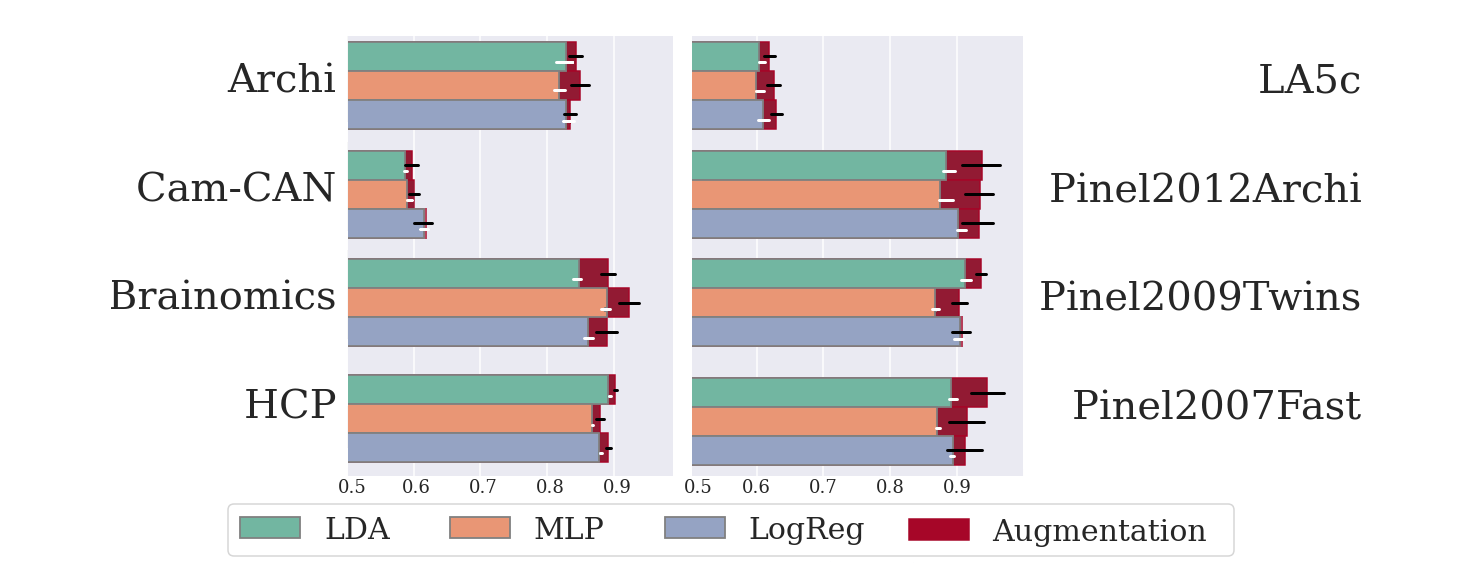
\includegraphics[width=\textwidth]{figures/condica/accuracy_all_datasets_v5.png}
\caption{\textbf{Accuracy of models for eight multi-contrast datasets.} Cross
  validated accuracy of two linear (LDA and LogReg) and one non-linear
  classifier (MLP) with or without using data augmentation.
  %
  The improvement yielded by data augmentation is displayed in red.
  %
  Black error bars indicate standard deviation across splits while white error bars indicate standard deviation across splits with no augmentation.}
\label{Fig4}
\end{figure}
%

Lastly, we provide a sensitivity analysis on the number of components used in
CondICA in figure~\ref{condica:sensitivity:fig}.
CondICA gives good performance for numbers of components between 800 and 1000
components. In all experiments we used $k=900$ components.

\begin{figure}
  \centerline{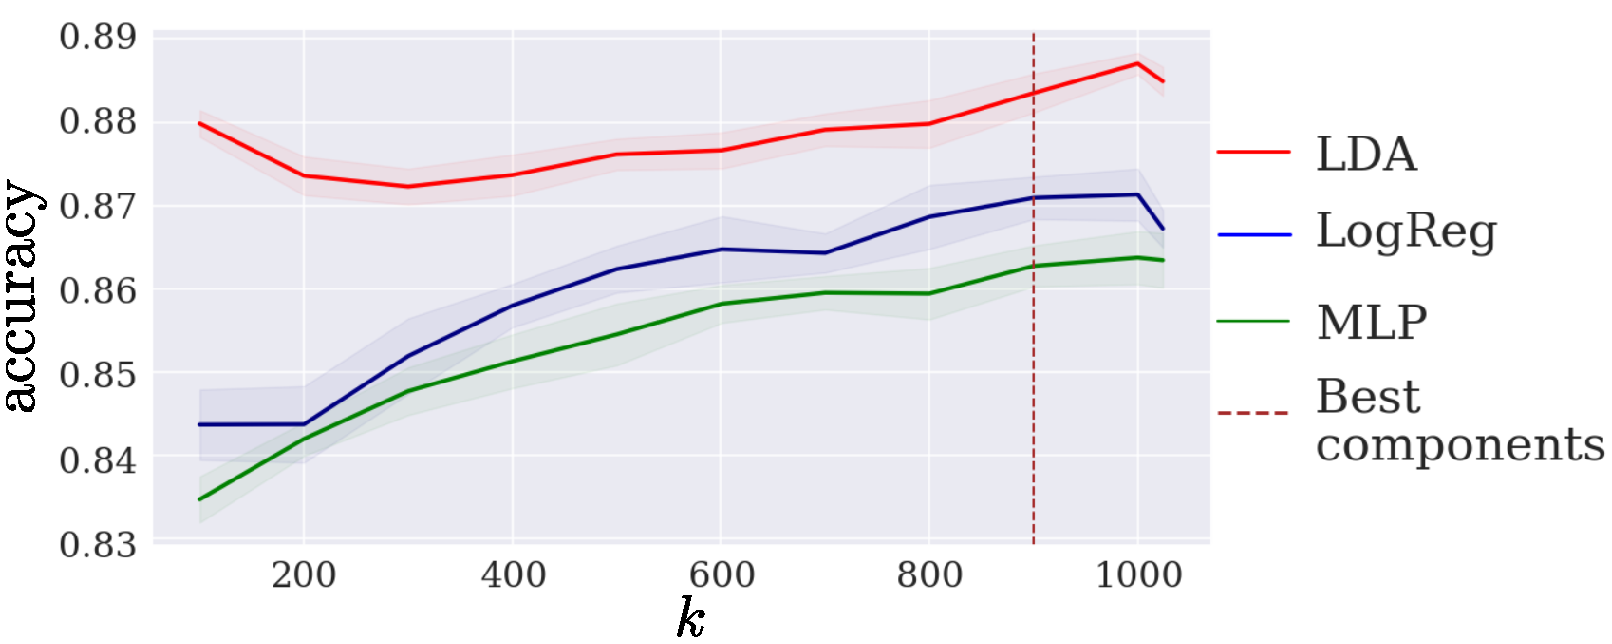
\includegraphics[width=0.8\textwidth]{figures/condica/sensitivity.pdf}}
  \caption{\textbf{Accuracy of augmented discriminative models when
      varying $k$.} We use 100 train subjects from the HCP task dataset to train Conditional ICA with $k$ components and generate $200$ fake subjects.
    Classifiers are trained on the train and fake subjects and tested on the
    left-out 687 subjects. We repeat the procedure
    for various values of $k$ using 5 random splits per value and
    report the mean accuracy across splits as a function of $k$.
    The dotted line represents the number of components that has been
    used in our experiments ($k=900$).
  }
  \label{condica:sensitivity:fig}
\end{figure}






\section{Conclusion}
Conditional ICA produces samples that cannot be distinguished from actual rest fMRI data by linear as well as non-linear classifiers, showing that it captures higher-order statistics than naive ICA-based generators.
%
When Conditional ICA is used as a data augmentation method, it yields consistent
improvement in classification accuracy: on 8 tasks fMRI datasets, we observe
increase in accuracy between 1\% and 5\% depending on the dataset and the
classifier used.
Importantly, this performance was obtained without any fine-tuning of
the method, showing its reliability. One can also notice that our experiments cover datasets with different cardinalities, from tens to thousand, and different baseline prediction accuracy.

The systematic performance improvement CanICA yields
makes it a promising candidate for data augmentation in a wide range of
contexts. Future work may focus on its applicability to other decoding tasks
such as the diagnosis of Autism Spectrum Disorder
(ASD)~\cite{eslami2019asd,eslami2019auto,dvornek2017identifying} or
Attention-Deficit/Hyperactivity Disorder detection (ADHD)~\cite{mao2019spatio}. Other extensions of the present work concern the adaptation to
individual feature (e.g. age) prediction where
fMRI has shown some potential.
%
